\documentclass[12pt,twoside,a4paper,BCOR=12mm,chapterprefix=true]{scrbook}

\pdfsuppresswarningpagegroup=1 %suppress multiple page groups warning of pdflatex
% --------------------------------------
% Packages
% --------------------------------------
\usepackage{tikz}
\usetikzlibrary{shapes.geometric, arrows, positioning}
\tikzstyle{block} = [rectangle, draw, text centered, minimum height=3em, minimum width=4em]
%\tikzstyle{block} = [draw, thick, rectangle, minimum height=1cm, minimum width=2cm, text centered, text width=2.5cm]
\tikzstyle{arrow} = [thick,->,>=stealth]
\usepackage[top=31mm, left=25mm, right=25mm, bottom=30mm, headsep=8mm, footskip=12mm]{geometry}

\usetikzlibrary{positioning, fit}
\usetikzlibrary{shapes.multipart}
\usepackage[english]{babel}    		
\usepackage[utf8]{inputenc}         		% use of unicode (non ASCII) characters eg: ä, ö, ü
\usepackage{graphicx}						% simple use of graphics

\graphicspath{{Images/}}			    
\usepackage{siunitx}  						% SI-units
\usepackage{amsmath}  						% handling of mathematical formulas (center)
\usepackage{amsfonts}
\usepackage{amssymb}
\usepackage{scrlayer-scrpage}       		% for headers
\usepackage{float}							% force placement of figure at place in code with argument H		
\usepackage{color}
\usepackage[dvipsnames]{xcolor}
\usepackage{listings}
\usepackage{transparent}
\usepackage{enumitem} 						% control layout of \itemize (no indent)
%\usepackage{tikz}              % for drawing figures
\usepackage{graphicx} % For diagrams
\usepackage{subcaption}    % For subfigures and captions
%\usepackage[margin=1in]{geometry} % Adjust margins for more space
\usepackage{booktabs} % For nicer tables
\usepackage{longtable} % For tables that span multiple pages
\usepackage{svg} % For including svg files
\setitemize{leftmargin=*}
\usepackage[table,xcdraw]{xcolor}
\usepackage{multirow}						% multi rows for tabulars	 
\usepackage{multicol}  						% multi cols for tabulars
\usepackage{setspace}						% enables different line spacings
\usepackage{pdfpages}						% include pdf-documents in latex
\usepackage[Sonny]{fncychap}  				% chapter heading styles. There are Sonny, Lenny, Glenn, Conny, Rejne, Bjarne, Bjornstrup.
 	% Displays the document in two columns, odd-numbered pages to the right								
\usepackage{braket} 						% bra-ket notation
%\usepackage{tabu} 							% Tabellen-Paket: Abstand zwischen Text und Linie
\usepackage{lipsum}							% for Lorem ipsum ... dummy text
\usepackage{scrhack}
\usepackage[titletoc]{appendix}
\usepackage[version=4]{mhchem}
%subfigure is deprecated, use subcaption instead
\usepackage{subcaption}
% \usepackage{layouts}						% use only to get textwidth for export of figures
\usepackage{csquotes}
\usepackage{listings}
\usepackage[style=numeric, backend=biber, backref, maxbibnames=5,maxalphanames=1]{biblatex} % Include the biblatex package
\renewcommand*{\labelalphaothers}{}
\addbibresource{BibTeX/bibliography.bib} % Specify the bibliography file

\usepackage[colorlinks,linkcolor=black,citecolor=tumblauTitel,urlcolor=black]{hyperref} 									% refs with hyperlinks and colour, autoref etc
\usepackage[nameinlink]{cleveref}
% \hypersetup{pdfpagelayout=TwoColumnRight}
\usepackage{duckuments}

% --------------------------------------
% Biber settings
% --------------------------------------

\DeclareSourcemap{
  \maps[datatype=bibtex]{
    \map[overwrite]{
      \step[fieldsource=doi, final]
      \step[fieldset=issn, null]
      \step[fieldset=url, null]
      \step[fieldset=eprint, null]
    }
  }
}

\DeclareSourcemap{
  \maps[datatype=bibtex]{
    \map[overwrite]{
      \step[fieldsource=doi, final]
      \step[fieldset=urldate, null]
    }
  }
}

\DeclareSourcemap{
  \maps[datatype=bibtex]{
    \map{
      \step[fieldset=language, null]
    }
  }
}

\DeclareSourcemap{
  \maps[datatype=bibtex]{
    \map{
      \step[fieldset=note, null]
    }
  }
}


% --------------------------------------
% Code Patch
% --------------------------------------

% color def

\definecolor{darkred}{rgb}{0.6,0.0,0.0}
\definecolor{darkgreen}{rgb}{0,0.50,0}
\definecolor{lightblue}{rgb}{0.0,0.42,0.91}
\definecolor{orange}{rgb}{0.99,0.48,0.13}
\definecolor{grass}{rgb}{0.18,0.80,0.18}
\definecolor{pink}{rgb}{0.97,0.15,0.45}

% listings

% General Setting of listings
\lstset{
  aboveskip=1em,
  breaklines=true,
  abovecaptionskip=-6pt,
  captionpos=b,
  escapeinside={\%*}{*)},
  frame=single,
  numbers=left,
  numbersep=15pt,
  numberstyle=\tiny,
}
% 0. Basic Color Theme
\lstdefinestyle{colored}{ %
  basicstyle=\ttfamily,
  backgroundcolor=\color{white},
  commentstyle=\color{green}\itshape,
  keywordstyle=\color{blue}\bfseries\itshape,
  stringstyle=\color{red},
}
% 1. General Python Keywords List
\lstdefinelanguage{PythonPlus}[]{Python}{
  morekeywords=[1]{,as,assert,nonlocal,with,yield,self,True,False,None,} % Python builtin
  morekeywords=[2]{,__init__,__add__,__mul__,__div__,__sub__,__call__,__getitem__,__setitem__,__eq__,__ne__,__nonzero__,__rmul__,__radd__,__repr__,__str__,__get__,__truediv__,__pow__,__name__,__future__,__all__,}, % magic methods
  morekeywords=[3]{,object,type,isinstance,copy,deepcopy,zip,enumerate,reversed,list,set,len,dict,tuple,range,xrange,append,execfile,real,imag,reduce,str,repr,}, % common functions
  morekeywords=[4]{,Exception,NameError,IndexError,SyntaxError,TypeError,ValueError,OverflowError,ZeroDivisionError,}, % errors
  morekeywords=[5]{,ode,fsolve,sqrt,exp,sin,cos,arctan,arctan2,arccos,pi, array,norm,solve,dot,arange,isscalar,max,sum,flatten,shape,reshape,find,any,all,abs,plot,linspace,legend,quad,polyval,polyfit,hstack,concatenate,vstack,column_stack,empty,zeros,ones,rand,vander,grid,pcolor,eig,eigs,eigvals,svd,qr,tan,det,logspace,roll,min,mean,cumsum,cumprod,diff,vectorize,lstsq,cla,eye,xlabel,ylabel,squeeze,}, % numpy / math
}
% 2. New Language based on Python
\lstdefinelanguage{PyBrIM}[]{PythonPlus}{
  emph={d,E,a,Fc28,Fy,Fu,D,des,supplier,Material,Rectangle,PyElmt},
}
% 3. Extended theme
\lstdefinestyle{colorEX}{
  basicstyle=\ttfamily,
  backgroundcolor=\color{white},
  commentstyle=\color{darkgreen}\slshape,
  keywordstyle=\color{blue}\bfseries\itshape,
  keywordstyle=[2]\color{blue}\bfseries,
  keywordstyle=[3]\color{grass},
  keywordstyle=[4]\color{red},
  keywordstyle=[5]\color{orange},
  stringstyle=\color{darkred},
  emphstyle=\color{pink}\underbar,
}

%--------------------------------------
% Layout
%--------------------------------------

\setlength{\parindent}{0pt} 				% set paragraph indent to 0

%--------------------------------------
% Typeface (Schriftbild)
%--------------------------------------
%\renewcommand{\familydefault}{\sfdefault}	% serif free font
\onehalfspacing       						% 1,5-line spacing
%\setlength{\parindent}{0pt} 				% set paragraph indent to 0

% --------------------------------------

\clubpenalty = 10000 						% no clubs (Schusterjungen)
\widowpenalty = 10000 						% no widows (Hurenkinder)
\displaywidowpenalty = 10000				% no widows before formulas

% --------------------------------------
% Captions
% --------------------------------------

\setkomafont{caption}{\itshape}				% Font for caption
\setkomafont{captionlabel}{\upshape}		% Font "Figure#"
%\setcapindent{0.cm}						% indent for captions
\renewcommand{\textfraction}{0.15} 			% minimum amount of text on page for figure/table ... placement by float 
\renewcommand{\topfraction}{.85}     		% maximum percentage of page that can be used for figures/tables ...

% --------------------------------------

\raggedbottom

% --------------------------------------
% Header
% --------------------------------------

\pagestyle{scrheadings} 					% normal header
%\renewcommand*{\chaptermarkformat}{%
%\chapappifchapterprefix{\ }\thechapter\autodot: }  %places a ":" after Chapter# 
\KOMAoptions{headsepline=0.6pt:\textwidth}			% Line 0.6pt and as wide as the text
\renewcommand{\headfont} 					% Normal font in header

% --------------------------------------
% Font for captions	
% --------------------------------------

\setkomafont{caption}{\rmfamily}			% Changes "Sonny" (sf-family) to rm-family
\setkomafont{chapter}{\rmfamily\large\bfseries}
\setkomafont{chapterentry}{\rmfamily\large\bfseries}
%\RedeclareSectionCommand[tocnumwidth=1.5em]{chapter} % would make
\setkomafont{section}{\rmfamily\large\bfseries}
\setkomafont{subsection}{\rmfamily\large\bfseries}
\setkomafont{paragraph}{\rmfamily\large\bfseries}
\ChNameVar{\Large}
\ChTitleVar{\Large}

% --------------------------------------
% Own definitions
% --------------------------------------

% changes autoref for chapter to uppercase (also needed for section, subsection etc)
%\addto\extrasenglish{%
%	\renewcommand{\chapterautorefname}{Chapter}%
%}

\sisetup{separate-uncertainty=true}

\renewcommand{\sectionautorefname}{Section}
\renewcommand{\subsectionautorefname}{Section}
\renewcommand{\subsubsectionautorefname}{Section}

%\addto\extrasenglish{ 	\renewcommand{\sectionautorefname}{Section} 	\let\subsectionautorefname\sectionautorefname 	\let\subsubsectionautorefname\sectionautorefname }



% --------------------------------------

\definecolor{cblau}{rgb}{0.69,0.89,1.0}		% blue
\definecolor{tumblauTitel}{cmyk}{1.0,0.43,.0,.1} % Tum-blue

% --------------------------------------

\newcommand{\moly}{$\text{MoS}_2$}
\newcommand{\woly}{$\text{WS}_2$}
\newcommand{\molyd}{$\text{MoS}_2~$}
\newcommand{\wolyd}{$\text{WS}_2~$}
\newcommand{\HS}{$\text{MoS}_2$/$\text{WS}_2$}
\newcommand{\HSd}{$\text{MoS}_2$/$\text{WS}_2~$}
\newcommand{\etal}{\textit{et al.}}
\newcommand{\etald}{$\textit{et al.}~$}
\newcommand{\dr}{$\Delta\text{R}/\text{R}~$}
\newcommand{\Fd}{$\vec{F}~$}
\newcommand{\F}{$\vec{F}$}
\newcommand{\pd}{$\vec{p}~$}
\newcommand{\p}{$\vec{p}$}
\newcommand{\kit}{$\textit{\textbf{k}}$}
\newcommand{\kitm}{\textit{\textbf{k}}}
\newcommand{\itm}[1]{\textit{\textbf{#1}}}

% --------------------------------------

\newcommand{\muW}[1]{\SI{#1}{\micro\watt}}
\newcommand{\K}[1]{\SI{#1}{\kelvin}}
\newcommand{\nm}[1]{\SI{#1}{\nano\meter}}
\newcommand{\V}[1]{\SI{#1}{\volt}}
\newcommand{\eV}[1]{\SI{#1}{\electronvolt}}
\newcommand{\mum}[1]{\SI{#1}{\micro\meter}}
\newcommand{\meV}[1]{\SI{#1}{\milli\electronvolt}}
\newcommand{\cm}[1]{\SI{#1}{\centi\meter^{-1}}}
\newcommand{\muWmum}[1]{\SI{#1}{\micro\watt\per\micro\meter^{2}}}
\newcommand{\kWcm}[1]{\SI{#1}{\kilo\watt\per\centi\meter^{2}}}
\newcommand{\percent}[1]{\SI{#1}{\percent}}
\newcommand{\meVV}[1]{\SI[per-mode=symbol]{#1}{\milli\electronvolt\per\volt}}
\newcommand{\angstrom}[1]{\SI{#1}{\angstrom}}
\newcommand{\ns}[1]{\SI{#1}{\nano\second}}
\newcommand{\um}[1]{\SI{#1}{\micro\meter}}


% --------------------------------------

\DeclareSIUnit{\nothing}{\relax}

%relative wavenumber
\DeclareSIUnit{\rel}{rel}
%celcius
\DeclareSIUnit{\celcius}{\degreeCelsius}

% --------------------------------------
% Back references
% --------------------------------------


% --------------------------------------

\def\logooffset{271}
\def\phylogo{
\includegraphics[height=15.605mm]{ph-logo.pdf}}
\def\wsilogo{
\includegraphics[height=15.605mm]{wsi_logo.jpg}}
\def\tumlogo{
\includegraphics[height=15.605mm]{Tum_logo.png}} % optional MSE logo
\def\deadline{August 2024} 					% month and year of submission
\def\title{Optics and Optomechanics of Freely Suspended \ce{MoS2} Monolayers}   				% title of the thesis
\def\author{Benedict Brouwer}							% your name
\def\typeOfThesis{Bachelor's Thesis}   		

\renewcommand\maketitle{
\begin{titlepage}
	\vspace*{1.0cm}%
	\noindent
	\begin{picture}(0,0)(25,\logooffset)
    	\put(25,272){\phylogo}					% 25,272
    	\put(90,272){\wsilogo}
    	\put(410,272){\tumlogo}					% 176,272
	\end{picture}%
  
	\vspace*{1.5cm}%

	\noindent\fontsize{12}{16}\selectfont\rmfamily Walter Schottky Institute\\
	School of Natural Sciences\\
	Technical University of Munich
	
	\vspace*{2cm} 
	% Anpassung der Schriftgroesse des Titels exakt 15 - Durchschuss 20
	\begin{center}
		{\color{tumblauTitel}
		\noindent\fontsize{20.74}{26}\selectfont\rmfamily\textbf{\title}
		}

		\vspace{2cm}
		% author
		\noindent\fontsize{17.28}{22}\selectfont\textbf{\author}
  
		\vspace{0.5cm}
		\noindent\fontsize{12}{16}\selectfont\rmfamily\typeOfThesis
		%\vspace{20\baselineskip}

		\vspace{2cm}
		Supervisor: \\
		\noindent\fontsize{12}{16}\selectfont\rmfamily\textbf{Prof. Dr. Alexander W. Holleitner} \\
		Chair of Nanotechnology and Nanomaterials

		\vspace{0.5cm}

		Second Examiner: \\
		\noindent\fontsize{12}{16}\selectfont\rmfamily{PD Dr. Hans-Gregor Hübl} \\



    	\vfill
    	\noindent\deadline
	\end{center}
\end{titlepage}
} 

% --------------------------------
%   DOCUMENT
% --------------------------------

\begin{document}
\selectlanguage{english}
\pagenumbering{Roman} 	
					% roman numbers for abstract and toc

% --------------------------------------

\frontmatter								% roman page numbering
\maketitle

% --------------------------------
%   Include abstracts
% --------------------------------

\newpage
\addchap*{Abstract}
%\vspace*{1cm}

Thesis template from the ZNN, updated for Biblatex and Biber.


%\selectlanguage{german}
%\addchap*{Zusammenfassung}
\selectlanguage{german}
%\vspace*{2cm}
%\thispagestyle{empty}

German Abstract
%\selectlanguage{english}

% --------------------------------
%   TABLE OF CONTENTS
% --------------------------------

\tableofcontents

% --------------------------------------

\mainmatter									% arabic page numbering

% --------------------------------
%   INTRODUCTION
% --------------------------------

\chapter{Introduction}
\label{chap:introduction}


to cite use \\autocite\{\} to reference use \\cref\{\}

% -------------------------------
%   Descripton of theory
% -------------------------------

\chapter{Theoretical concepts}\label{cha:theory}

In \autoref{cha:theory} we will talk about theory. We start with lorem ipsum in \autoref{sec:this_a_sec}. Then continue with \molyd and \wolyd in \autoref{subsec:theorie_PL} and so on.
% Our text is \printinunitsof{in}\prntlen{\textwidth}\\ wide! % needs \usepackage{layouts}

\section{Referencing figures}\label{sec:this_a_sec}

In \autoref{fig:MoS2_schematic} one can see some nice pictures.


\unpacklipsum[2]\lipsumexp

\begin{figure}[t]
	\includegraphics[width=1\textwidth,keepaspectratio=true]{Images/MoS2_2.pdf}
	\caption[]{\textbf{(a)} Nice picture 1 \textbf{(b)}Nice picture 2}
	\label{fig:MoS2_schematic}
\end{figure}

\subsection{Stuff with \texorpdfstring{\moly}{MoS2} and \texorpdfstring{\woly}{WS2}}\label{subsec:theorie_PL} % \textorpfdstring needed to handle math symbols in section names and give ASCII alternative

\unpacklipsum[1-1]{}\lipsumexp

\subsection{Next section}\label{sec:next_sec}

One can also show figures where they where plaaced in the tex file or if not possible on top etc. by giving [!ht] as arguments.

\begin{figure}[!htb]
	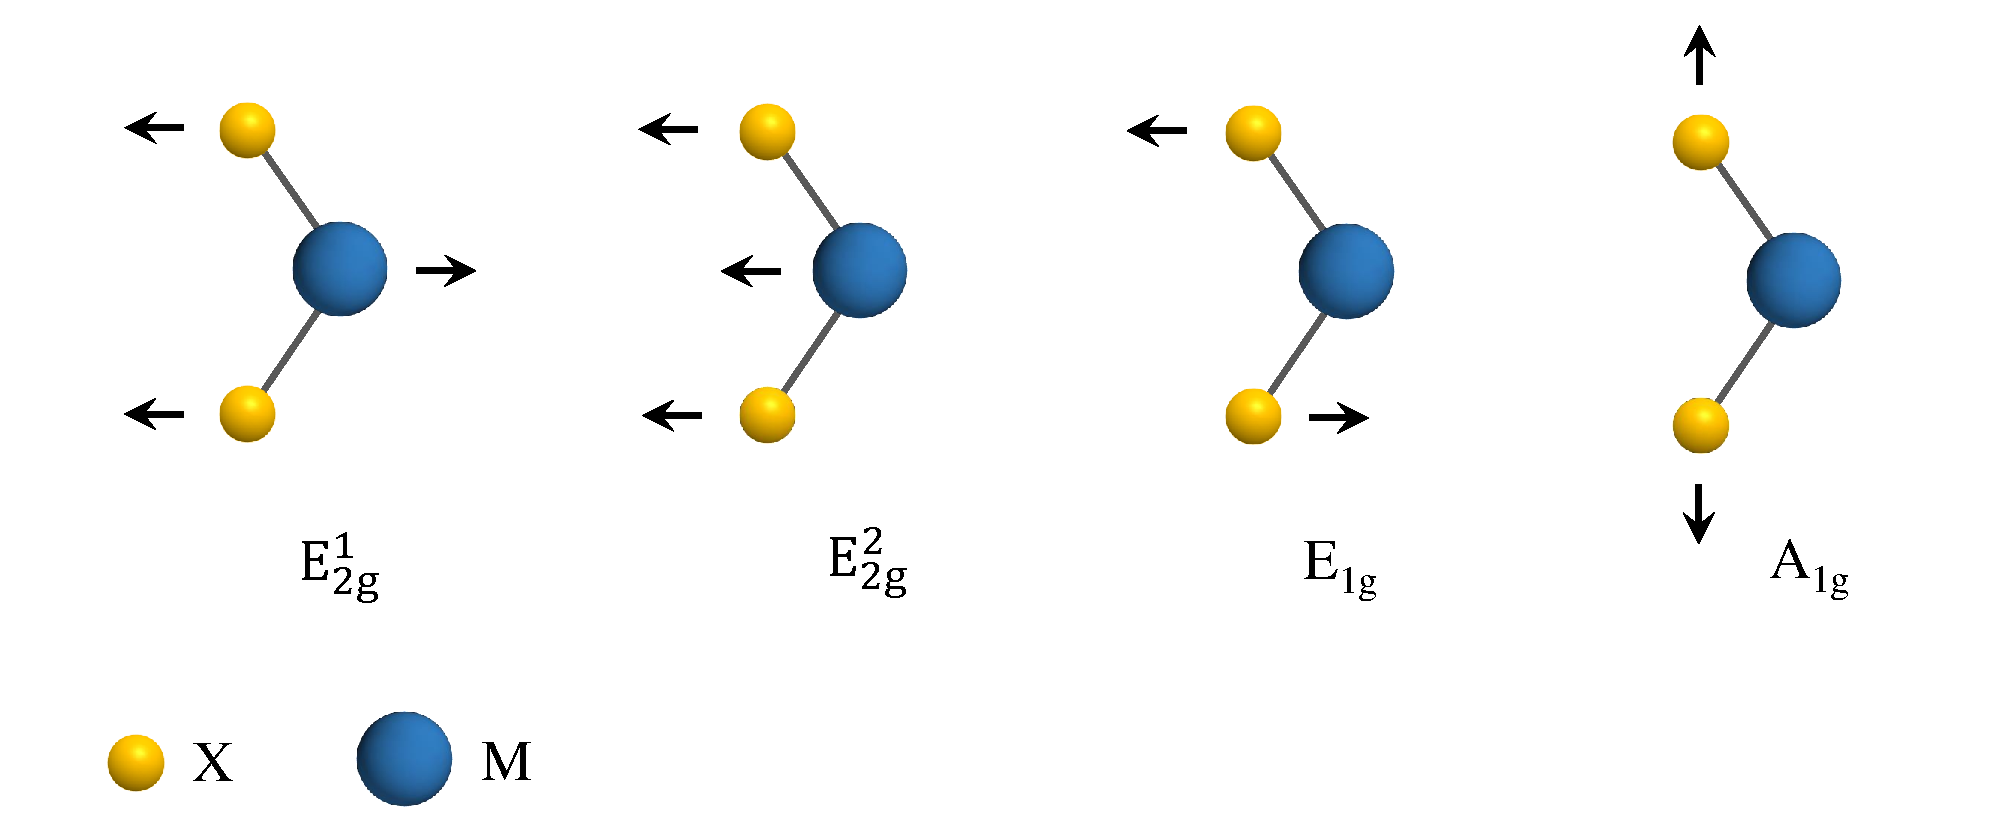
\includegraphics[width=1\textwidth,keepaspectratio=true]{Images/Ramanmoden.pdf}
	\caption[]{Second nice figure: Sketch of the atomic displacement for the Raman active phonon modes at the $\Gamma$-point in the monolayer $D_{3h}^1$ symmetry.}
	\label{fig:ramanmodes}
\end{figure}

\unpacklipsum[2-3]{}\lipsumexp

\newpage

\section{The second section}\label{sec:the_sec_sec}

\unpacklipsum[3]{}\lipsumexp

\subsection{Equations and referencing}\label{subsec:formulas}

In the following we show Equations \ref{eq:fractions_propto_exp} to \ref{eq:sig_ext}. You should look at \autoref{eq:polarisation}!

\begin{equation}\label{eq:fractions_propto_exp}
	\frac{I\left(A^-\right)}{I\left( A\right)}
	=\frac{\Gamma_{\text{A}^-}N_{\text{A}^-}}{\Gamma_\text{A}N_{\text{A}}}\propto\frac{\Gamma_{\text{A}^-}}{\Gamma_{\text{A}}}\frac{1}{n_e}\exp{\left(\frac{\text{E}_{\text{A}^-}}{k_{\text{B}}\text{T}}\right)}
\end{equation}

\begin{equation}\label{eq:oplus}
	\Gamma=A_{1g}\oplus 2A_{2u}\oplus B_{1u}\oplus 2B_{2g}\oplus E_{1g}\oplus 2E_{1u}\oplus E_{2u}\oplus 2E_{2g}.
\end{equation}

\begin{equation}\label{eq:permittivity}
	m^*\dfrac{d^2x}{dt^2}+\dfrac{m^*}{\tau}\dfrac{dx}{dt}=-eE_0e^{-i\omega t}.
\end{equation}

\begin{equation}\label{eq:solution_Drude}
	x(t)=\dfrac{e}{m^*}\dfrac{1}{\omega(\omega +i\frac{1}{\tau})}E_0e^{-i\omega t}
\end{equation}

\begin{equation}\label{eq:polarisation}
	\textbf{P}=\epsilon_0\chi \textbf{E}=n_V\textbf{p}_{\text{el}},
\end{equation}

\begin{equation}\label{eq:approx_permittivity}
\varepsilon_r(\omega)\approx 1-\dfrac{\omega_p^2}{\omega^2},~~~~\varepsilon_i(\omega)\approx \dfrac{\omega_p^2}{\omega^3}\Gamma.
\end{equation}

\begin{align}
	\sigma_{\text{ext}}&=\dfrac{2\pi}{|\textbf{k}|^2}\sum\limits_{L=1}^{\infty}(2L+1)\text{Re}\left\lbrace a_L+b_L \right\rbrace\label{eq:sig_ext_sum}\\
	\sigma_{\text{sca}}&=\dfrac{2\pi}{|\textbf{k}|^2}\sum\limits_{L=1}^{\infty}(2L+1)(|a_L|^2+|b_L|^2)\label{eq:sig_sca_sum}\\
	\sigma_{\text{abs}} &=\sigma_{\text{ext}}-\sigma_{\text{sca}}\label{eq:sig_abs}
\end{align}

We can even cite the equations in the align environment above. Like \autoref{eq:sig_ext_sum} and \autoref{eq:sig_sca_sum}

\begin{equation}\label{eq:sig_ext}
	\sigma_{\text{ext}}=12\pi\epsilon_m^{3/2}R^3\dfrac{\omega}{c}\dfrac{\varepsilon_i(\omega)}{\left[\varepsilon_r(\omega)+2\epsilon_m\right]^2+\varepsilon_i(\omega)^2},
\end{equation}

\subsection{Citation}\label{subsec:more_theory}

We will cite a lot in a theory chapter, but the best source is \autocite{gross_festkorperphysik_2018} but of course we cannot forget about \cite{fox_optical_2010,fox_quantum_2006}!

\unpacklipsum[4]{}\lipsumexp


% -------------------------------
%   Descripton of experimental part
% -------------------------------

\chapter{Experimental Procedures}\label{cha:experimental_procedures}

\chapter{Development of the FPGA firmware for the SFH}\label{cha:development}
The firmware developed in this thesis for the three Artix-7 FPGAs, located on the iFTDC as described in Section \ref{sec:iFTDC}, must perform several functionalities.
The main tasks of the firmware are to configure the Citiroc1A ASIC, explained in Section \ref{sec:configuration},
 communicaton with the controlling coputer via ethernet and the IPBUS protocol and a provisional readout of the time triggerd data from the Citiroc1A ASIC.
\section{The IPBUS protocol}
The IPBUS protocol used for the communication between the FPGA and the controlling computer is a simple protocol for controlling IP-aware hardware devices with a 32 bit read and write bus using UDP as the transport protocol.\autocite{IPBUS_article}
\newline
The IPBUS protocol defines a read and write command enabling successful write and read operations of a 32 bit register, with a 32 bit address in the FPGA.    
\newline
The commands can be issued on the controling computer with the $\mu$HAL library, which allowes the user to issue read and write commands with a python script and an XML file defining the address of the registers.\autocite{IPBUS_article}
\newline
The address space inside the FPGA is defined in the firmware. The address space is divided into seprate address spaces for each of the slaves by the leading bits of the address.
For some slaves, the address space is further divided into subspaces for the different registers of the slave. 
\section{Configuration of the Citiroc1A ASIC}
The configuration of the slow control and probe registers of the Citiroc1A ASIC,
 along with the verification of this configuration, is handled by two state machines. Both state machines control a single random access memory (RAM) with a depth of 64 addresses, where each address stores 32 bits of data.
The state machiens inturn are controled by the status and control register which can be written by the controlling computer via the ipbus protocol.
\subsection{Status and control register}
herre i will explain the status and control register
\subsection{Configuration state machine}
\begin{figure}[H]
    \centering
    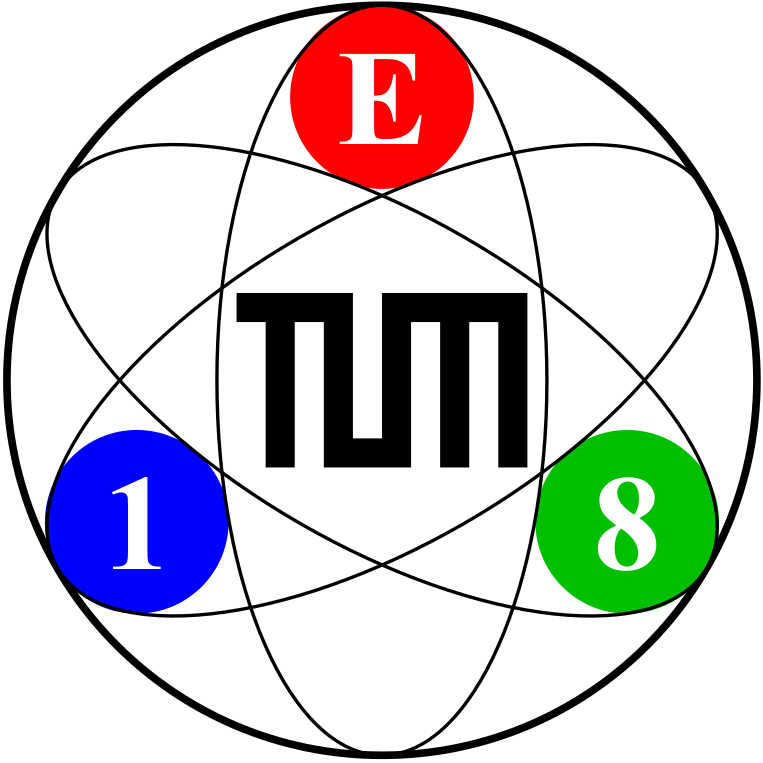
\includegraphics[width=\textwidth]{E18Logo.png}%{CONFIGSMALLdiagram2.png}
    \caption{State machine for the configuration of the Citiroc1A ASIC.}
    \label{fig:Configuration_state_machine}
\end{figure}
\subsection{Verification state machine}
\begin{figure}[H]
    \centering
    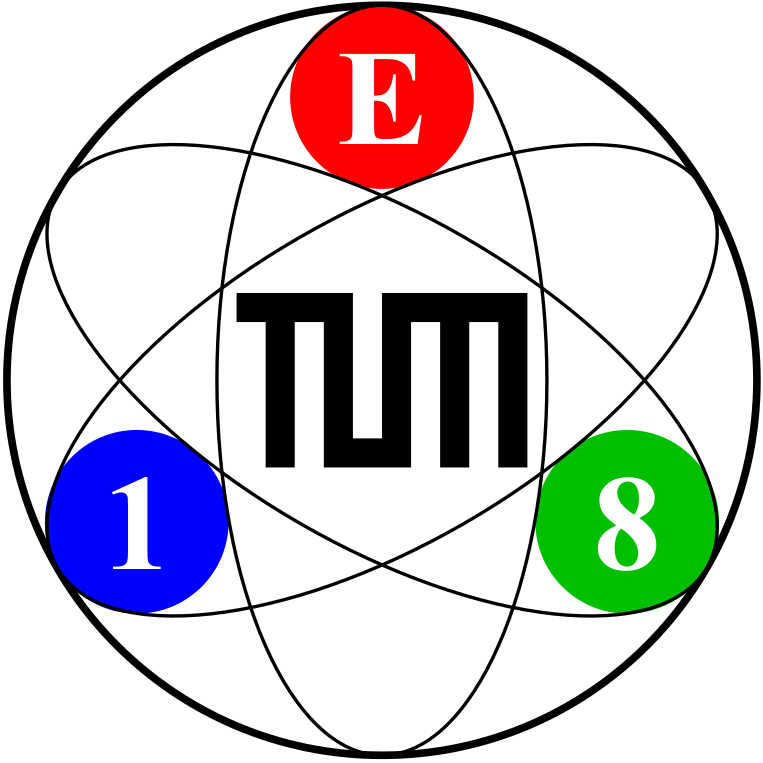
\includegraphics[width=\textwidth]{E18Logo.png}%{smallVerifacationdiagrammod.png}
    \caption{State machine for the verification of the configuration of the Citiroc1A ASIC.}
    \label{fig:Verification_state_machine}
\end{figure}



% -------------------------------
%   Descripton of dicussion
% -------------------------------
\chapter{Results}\label{cha:results}\


%\chapter{Discussion}\label{cha: discussion}

Discussion

% -------------------------------
%   Conclusion and Outlook
% -------------------------------

\chapter{Conclusion and Outlook}

\section{Conclusion}

Conclusion

\section{Outlook}

Outlook       

% -------------------------------
%   Appendix
% -------------------------------

\begin{appendices}							% start of appendix: numbering in capsize letters
\chapter{Configurable Registers of the Citiroc1A ASIC}\label{cha:Citiroc1A_register}

\begin{longtable}{|p{6cm}|p{1cm}|p{1.4cm}|p{1.8cm}|p{5cm}|}
    
    \caption{Configurable registers of the slow control register\autocite{InternalcommunicationKarl} \label{tab:slow_control_register}} \\ \hline
    \hline
\textbf{Field} & \textbf{Bits} & \textbf{Default} & \textbf{Position} & \textbf{Description} \\ \hline
\endfirsthead

\hline
\textbf{Field} & \textbf{Bits} & \textbf{Default} & \textbf{Position } & \textbf{Description} \\ \hline
\endhead

\hline
\multicolumn{5}{r}{{Configurable registers of the slow control register continued on next page}} \\
\endfoot

\hline
\endlastfoot

% channel_thr_time
\multicolumn{5}{|l|}{\textcolor{red}{Register:channel\_thr\_time}} \\ \hline
ch\_0       & 4  & 0 & 0   & Channel-dependent 4-bit threshold for time discriminator. \\ \hline
 $\vdots$ & &   &  & \\ \hline % Vertical dots for skipped channels
%\multicolumn{5}{|l|}{\emph{See below for common 10-bit threshold.}} \\ \hline
ch\_31      & 4  & 0 & -   & - \\ \hline
\multicolumn{5}{|l|}{\textcolor{red}{Register:channel\_thr\_charge }} \\ \hline
% channel_thr_charge
ch\_0     & 4  & 0 & 128 & Channel-dependent 4-bit threshold for charge discriminator. \\ \hline
%\multicolumn{5}{|l|}{\emph{See below for common 10-bit threshold.}} \\ \hline
$\vdots$ & &   &  & \\ \hline % Vertical dots for skipped channels
 ch\_31    & 4  & 0 & -   & - \\ \hline

% discriminator_power
\multicolumn{5}{|l|}{\textcolor{red}{Register:discriminator\_power}} \\ \hline
discriminator\_charge\_en      & 1  & 0 & 256 & Enable charge discriminator. \\ \hline
discriminator\_charge\_pp      & 1  & 0 & -   & Power pulse for charge discriminator. \\ \hline
discriminator\_latched\_output & 1  & 0 & -   & 1: latched, 0: direct output. \\ \hline
discriminator\_time\_en        & 1  & 1 & -   & Enable time discriminator. \\ \hline
discriminator\_time\_pp        & 1  & 1 & -   & Power pulse for time discriminator. \\ \hline


4bit\_dac\_charge\_en          & 1  & 0 & 261   & Enable 4-bit charge DAC. \\ \hline
4bit\_dac\_charge\_pp          & 1  & 0 & -   & Power pulse for 4-bit charge DAC. \\ \hline
4bit\_dac\_time\_en            & 1  & 1 & -   & Enable 4-bit time DAC. \\ \hline
4bit\_dac\_time\_pp            & 1  & 1 & -   & Power pulse for 4-bit time DAC. \\ \hline

% channel_discriminator_mask
%\multicolumn{5}{|l|}{\emph{Register:channel\_discriminator\_mask } \\ \hline
 ch\_0 & 1  & 1 & 265 & 0: masked, 1: unmasked. \\ \hline
 $\vdots$ & &   &  & \\ \hline % Vertical dots for skipped channels
ch\_31 & 1  & 1 & - & - \\ \hline

% track_and_hold_power
\multicolumn{5}{|l|}{\textcolor{red}{Register:track\_and\_hold\_power}} \\ \hline
high\_gain\_pp & 1  & 0 & 297 & Enable high gain. \\ \hline
 high\_gain\_en & 1  & 0 & -   & - \\ \hline
 low\_gain\_pp  & 1  & 0 & -   & Power pulse for low gain. \\ \hline
 low\_gain\_en  & 1  & 0 & -   & Enable low gain. \\ \hline
 weak\_bias     & 1  & 0 & -   & 1: weak bias (600kHz max), 0: high bias (5MHz max). \\ \hline

% peak_detector_power
\multicolumn{5}{|l|}{\textcolor{red}{Register:peak\_detector\_power}} \\ \hline
 high\_gain\_pp & 1  & 0 & 302 & Enable high gain for peak detector. \\ \hline
 high\_gain\_en & 1  & 0 & - & - \\ \hline
 low\_gain\_pp  & 1  & 0 & - & Power pulse for low gain. \\ \hline
 low\_gain\_en  & 1  & 0 & - & Enable low gain for peak detector. \\ \hline

% select_peak_sensing
\multicolumn{5}{|l|}{\textcolor{red}{Register:select\_peak\_sensing}} \\ \hline
 high\_gain\_th & 1  & 0 & 306 & 0: peak detector, 1: track and hold. \\ \hline
 low\_gain\_th  & 1  & 0 & -   & - \\ \hline
peak\_sensing\_cell\_bypass          & 1  & 0 & -   & 0: cell active, 1: bypass peak sensing cell. \\ \hline
peak\_sensing\_external\_trigger     & 1  & 0 & -   & 0: internal trigger, 1: external trigger. \\ \hline

% shaper
\multicolumn{5}{|l|}{\textcolor{red}{Register:shaper}} \\ \hline
 fast\_shaper\_follower\_pp & 1  & 0 & 310 & Power pulse for fast shaper follower. \\ \hline
 fast\_shaper\_en           & 1  & 1 & -   & Enable fast shaper. \\ \hline
 fast\_shaper\_pp           & 1  & 1 & -   & Power pulse for fast shaper. \\ \hline
 low\_gain\_slow\_shaper\_pp & 1  & 0 & -   & Power pulse for low gain slow shaper. \\ \hline
 low\_gain\_slow\_shaper\_en & 1  & 0 & -   & Enable low gain slow shaper. \\ \hline
 low\_gain\_slow\_shaper\_time\_const & 3 & 0 & - & See the table above for values. \\ \hline
 high\_gain\_slow\_shaper\_pp & 1 & 0 & - & Power pulse for high gain slow shaper. \\ \hline
 high\_gain\_slow\_shaper\_en & 1 & 0 & - & Enable high gain slow shaper. \\ \hline
 high\_gain\_slow\_shaper\_time\_const & 3 & 0 & - & See the table above for values. \\ \hline

% (continue for all remaining parameters)
% Preamp Power Settings
\multicolumn{5}{|l|}{\textcolor{red}{Register:pre\_amp\_power}} \\ \hline
low\_gain\_weak\_bias       & 1  & 0 & 323 & 0: normal bias, 1: weak bias. \\ \hline
high\_gain\_pp             & 1  & 1 & -   & Power pulse for high gain preamp. \\ \hline
high\_gain\_en             & 1  & 1 & -   & Enable high gain preamp. \\ \hline
low\_gain\_pp              & 1  & 0 & -   & Power pulse for low gain preamp. \\ \hline
low\_gain\_en              & 1  & 0 & -   & Enable low gain preamp. \\ \hline
fast\_shaper\_low\_gain     & 1  & 0 & -   & 0: fast shaper on high gain. \\ \hline

% Input DAC Settings
\multicolumn{5}{|l|}{\textcolor{red}{Register:input\_dac}} \\ \hline
dac\_en                   & 1  & 1 & 329 & Input DAC for bias correction. \\ \hline
dac\_ref                  & 1  & 1 & -   & Voltage ref: 1 = internal 4.5V, 0 = internal 2.5V, depends on vdd\_dac. \\ \hline
ch\_0                     & 8  & 255 & - & VSipm = V\_HV - V\_DAC (check what makes sense here). \\ \hline
ch\_0\_en                  & 1  & 1 & -   & Enable channel 0 input DAC. \\ \hline
$\vdots$ & &   &  & \\ \hline
ch\_31                    & 8  & 255 & - & Same as ch\_0 for channel 31. \\ \hline
ch\_31\_en                 & 1  & 1 & -   & Enable channel 31 input DAC. \\ \hline

% Channel Preamp
\multicolumn{5}{|l|}{\textcolor{red}{Register:channel\_preamp}} \\ \hline
ch\_0\_hg                  & 6  & 62 & 619 & High gain preamp setting. \\ \hline
ch\_0\_lg                  & 6  & 0  & -   & Low gain preamp setting. \\ \hline
ch\_0\_ctest\_hg            & 1  & 0  & -   & 1: Connect injection capacitance for test signal. \\ \hline
ch\_0\_ctest\_lg            & 1  & 0  & -   & 1: Connect low gain injection capacitance. \\ \hline
ch\_0\_disable             & 1  & 0  & -   & 1 disables preamp for channel 0. \\ \hline
$\vdots$ & &   &  & \\ \hline
ch\_31\_hg                  & 6  & 62 & - & High gain preamp setting. \\ \hline
ch\_31\_lg                  & 6  & 0  & -   & Low gain preamp setting. \\ \hline
ch\_31\_ctest\_hg            & 1  & 0  & -   & 1: Connect injection capacitance for test signal. \\ \hline
ch\_31\_ctest\_lg            & 1  & 0  & -   & 1: Connect low gain injection capacitance. \\ \hline
ch\_31\_disable             & 1  & 0  & -   & 1 disables preamp for channel 0. \\ \hline
% Service Blocks
\multicolumn{5}{|l|}{\textcolor{red}{Register:service\_blocks}} \\ \hline
temp\_pp                  & 1  & 1 & 999   & Enable power pulse for temperature monitoring. \\ \hline
temp\_en                  & 1  & 1 & -   & Enable temperature monitoring. \\ \hline
band\_gap\_pp              & 1  & 1 & -   & Enable power pulse for band gap reference. \\ \hline
band\_gap\_en              & 1  & 1 & -   & Enable band gap reference. \\ \hline

% Threshold DAC
\multicolumn{5}{|l|}{\textcolor{red}{Register:threshold\_dac}} \\ \hline
charge\_dac\_en            & 1  & 0 & 1103 & Enable charge threshold DAC. \\ \hline
charge\_dac\_pp            & 1  & 0 & -   & Power pulse for charge threshold DAC. \\ \hline
time\_dac\_en              & 1  & 1 & -   & Enable time threshold DAC. \\ \hline
time\_dac\_pp              & 1  & 1 & -   & Power pulse for time threshold DAC. \\ \hline
charge\_threshold         & 10 & 0 & -   & Charge threshold value. \\ \hline
time\_threshold           & 10 & - & -   & Time threshold value (e.g., ~200 for 1 cell min, ~250 for 2 cells). \\ \hline

% OTAQ Power
\multicolumn{5}{|l|}{\textcolor{red}{Register:otaq\_power}} \\ \hline
high\_gain\_en             & 1  & 1 & 1127 & Enable high gain for OTAQ. \\ \hline
high\_gain\_pp             & 1  & 1 & -    & Power pulse for high gain OTAQ. \\ \hline
low\_gain\_en              & 1  & 0 & -    & Enable low gain for OTAQ. \\ \hline
low\_gain\_pp              & 1  & 0 & -    & Power pulse for low gain OTAQ. \\ \hline
debug\_probe\_en           & 1  & 1 & -    & Enable debug probe. \\ \hline
debug\_probe\_pp           & 1  & 1 & -    & Power pulse for debug probe. \\ \hline

% Input/Output
\multicolumn{5}{|l|}{\textcolor{red}{Register:input\_output}} \\ \hline
output\_buffer\_bias       & 1  & 0 & 1133 & Output OTA buffer bias: 0 = auto bias, 1 = force on. \\ \hline
val\_event\_receiver\_en    & 1  & 1 & -    & Enable validation event receiver. \\ \hline
val\_event\_receiver\_pp    & 1  & 1 & -    & Power pulse for validation event receiver. \\ \hline
raz\_chn\_en               & 1  & 1 & -    & Enable RAZ channel. \\ \hline
raz\_chn\_pp               & 1  & 1 & -    & Power pulse for RAZ channel. \\ \hline
digital\_output\_en        & 1  & 1 & -    & Enable digital multiplexed output. \\ \hline
or32\_output\_en           & 1  & 1 & -    & Enable OR32 output. \\ \hline
or32\_oc\_output\_en        & 1  & 1 & -    & Enable OR32 over-current output. \\ \hline
trigger\_polarity         & 1  & 0 & -    & Trigger polarity: 0 = positive (rising edge), 1 = negative (falling edge). \\ \hline
or32\_t\_oc\_en             & 1  & 1 & -    & Enable OR32 timeout over-current. \\ \hline
32\_triggers\_en           & 1  & 1 & 1143    & Enable 32 triggers. \\ \hline
\end{longtable}
\newpage
\begin{longtable}{|p{5cm}|p{2cm}|c|c|p{6cm}|}
    \caption{Configurable registers of the probe register\autocite{InternalcommunicationKarl} \label{tab:probe_register_tab}} \\ \hline
    
    \hline
    \textbf{Register}                & \textbf{Field} & \textbf{Bits} & \textbf{Position} & \textbf{Type} \\ 
    \hline
    \endfirsthead
    
    \hline
    \textbf{Register}                & \textbf{Field} & \textbf{Bits} & \textbf{Position} & \textbf{Type} \\ 
    \hline
    \endhead
    
    \hline
    \endfoot
    
    \hline
    \endlastfoot
    
    % Data rows
    out\_probe\_fast\_shaper       & ch\_0   & 1 & 0   & Analog - Out\_probe \\
                                   & $\vdots$ &   & $\vdots$ & \\ % Vertical dots for skipped channels
                                   & ch\_31  & 1 & 31  &  \\
    \hline
    out\_probe\_slow\_shaper\_lg  & ch\_0   & 1 & 32  & Analog - Out\_probe \\
                                   & $\vdots$ &   & $\vdots$ & \\ % Vertical dots for skipped channels
                                   & ch\_31  & 1 & 63  &  \\
    \hline
    digital\_probe\_peak\_sense\_lg & ch\_0   & 1 & 64  & Digital - Digital\_probe \\
                                   & $\vdots$ &   & $\vdots$ & \\ % Vertical dots for skipped channels
                                   & ch\_31  & 1 & 95   \\
    \hline
    out\_probe\_slow\_shaper\_hg  & ch\_0   & 1 & 96  & Analog - Out\_probe \\
                                   & $\vdots$ &   & $\vdots$ & \\ % Vertical dots for skipped channels
                                   & ch\_31  & 1 & 127 & \\
    \hline
    digital\_probe\_peak\_sense\_hg & ch\_0   & 1 & 128 & Digital - Digital\_probe \\
                                   & $\vdots$ &   & $\vdots$ & \\ % Vertical dots for skipped channels
                                   & ch\_31  & 1 & 159 &  \\
    \hline
    out\_probe\_preamp\_hg        & ch\_0   & 1 & 160 & Analog - Out\_probe \\
                                   & $\vdots$ &   & $\vdots$ & \\ % Vertical dots for skipped channels
                                   & ch\_31  & 1 & 191 &  \\
    \hline
    out\_probe\_preamp\_lg        & ch\_0   & 1 & 192 & Analog - Out\_probe \\
                                   & $\vdots$ &   & $\vdots$ & \\ % Vertical dots for skipped channels
                                   & ch\_31  & 1 & 223 &  \\
    \hline
    input\_dac\_probe             & ch\_0   & 1 & 224 & Analog - Out\_probe\_dac\_5V \\
                                   & $\vdots$ &   & $\vdots$ & \\ % Vertical dots for skipped channels
                                   & ch\_31  & 1 & 255 & \\
    
    \end{longtable}
\chapter{Fit parameters of the S-curve analysis}\label{cha:appendixFitPar}
\begin{table}[H]
    

    \resizebox{\textwidth}{!}{% Adjusts the table to the text width
    \begin{tabular}{|c|c|c|c|c|c|c|c|c|c|c|c|c|}
       
    \hline
    gain& FPGA 1 & FPGA 2 & Citiroc1A & Channel & $\mu$ & $\sigma$ & FPGA 1 & FPGA 2 & Citiroc1A & Channel & $\mu$ & $\sigma$ \\
    \hline

      57&ch\_0  & NAN & NAN & ch\_0  & NAN & NAN & ch\_0  & NAN & NAN & ch\_0  & NAN & NAN \\
        &ch\_1  & NAN & NAN & ch\_1  & NAN & NAN & ch\_1  & NAN & NAN & ch\_1  & NAN & NAN \\
        &ch\_2  & NAN & NAN & ch\_2  & NAN & NAN & ch\_2  & NAN & NAN & ch\_2  & NAN & NAN \\
        &ch\_3  & NAN & NAN & ch\_3  & NAN & NAN & ch\_3  & NAN & NAN & ch\_3  & NAN & NAN \\
        &ch\_4  & NAN & NAN & ch\_4  & NAN & NAN & ch\_4  & NAN & NAN & ch\_4  & NAN & NAN \\
        &ch\_5  & NAN & NAN & ch\_5  & NAN & NAN & ch\_5  & NAN & NAN & ch\_5  & NAN & NAN \\
        &ch\_6  & NAN & NAN & ch\_6  & NAN & NAN & ch\_6  & NAN & NAN & ch\_6  & NAN & NAN \\
        &ch\_7  & NAN & NAN & ch\_7  & NAN & NAN & ch\_7  & NAN & NAN & ch\_7  & NAN & NAN \\
        &ch\_8  & NAN & NAN & ch\_8  & NAN & NAN & ch\_8  & NAN & NAN & ch\_8  & NAN & NAN \\
        &ch\_9  & NAN & NAN & ch\_9  & NAN & NAN & ch\_9  & NAN & NAN & ch\_9  & NAN & NAN \\
        &ch\_10 & NAN & NAN & ch\_10 & NAN & NAN & ch\_10 & NAN & NAN & ch\_10 & NAN & NAN \\
        &ch\_11 & NAN & NAN & ch\_11 & NAN & NAN & ch\_11 & NAN & NAN & ch\_11 & NAN & NAN \\
        &ch\_12 & NAN & NAN & ch\_12 & NAN & NAN & ch\_12 & NAN & NAN & ch\_12 & NAN & NAN \\
        &ch\_13 & NAN & NAN & ch\_13 & NAN & NAN & ch\_13 & NAN & NAN & ch\_13 & NAN & NAN \\
        &ch\_14 & NAN & NAN & ch\_14 & NAN & NAN & ch\_14 & NAN & NAN & ch\_14 & NAN & NAN \\
        &ch\_15 & NAN & NAN & ch\_15 & NAN & NAN & ch\_15 & NAN & NAN & ch\_15 & NAN & NAN \\
        &ch\_16 & NAN & NAN & ch\_16 & NAN & NAN & ch\_16 & NAN & NAN & ch\_16 & NAN & NAN \\
        &ch\_17 & NAN & NAN & ch\_17 & NAN & NAN & ch\_17 & NAN & NAN & ch\_17 & NAN & NAN \\
        &ch\_18 & NAN & NAN & ch\_18 & NAN & NAN & ch\_18 & NAN & NAN & ch\_18 & NAN & NAN \\
        &ch\_19 & NAN & NAN & ch\_19 & NAN & NAN & ch\_19 & NAN & NAN & ch\_19 & NAN & NAN \\
        &ch\_20 & NAN & NAN & ch\_20 & NAN & NAN & ch\_20 & NAN & NAN & ch\_20 & NAN & NAN \\
        &ch\_21 & NAN & NAN & ch\_21 & NAN & NAN & ch\_21 & NAN & NAN & ch\_21 & NAN & NAN \\
        &ch\_22 & NAN & NAN & ch\_22 & NAN & NAN & ch\_22 & NAN & NAN & ch\_22 & NAN & NAN \\
        &ch\_23 & NAN & NAN & ch\_23 & NAN & NAN & ch\_23 & NAN & NAN & ch\_23 & NAN & NAN \\
        &ch\_24 & NAN & NAN & ch\_24 & NAN & NAN & ch\_24 & NAN & NAN & ch\_24 & NAN & NAN \\
        &ch\_25 & NAN & NAN & ch\_25 & NAN & NAN & ch\_25 & NAN & NAN & ch\_25 & NAN & NAN \\
        &ch\_26 & NAN & NAN & ch\_26 & NAN & NAN & ch\_26 & NAN & NAN & ch\_26 & NAN & NAN \\
        &ch\_27 & NAN & NAN & ch\_27 & NAN & NAN & ch\_27 & NAN & NAN & ch\_27 & NAN & NAN \\
        &ch\_28 & NAN & NAN & ch\_28 & NAN & NAN & ch\_28 & NAN & NAN & ch\_28 & NAN & NAN \\
        &ch\_29 & NAN & NAN & ch\_29 & NAN & NAN & ch\_29 & NAN & NAN & ch\_29 & NAN & NAN \\
        &ch\_30 & NAN & NAN & ch\_30 & NAN & NAN & ch\_30 & NAN & NAN & ch\_30 & NAN & NAN \\
        &ch\_31 & NAN & NAN & ch\_31 & NAN & NAN & ch\_31 & NAN & NAN & ch\_31 & NAN & NAN \\
        \hline
     
    \end{tabular}
    }
    \caption{Mean $\mu$ and standard deviation $\sigma$ of the noise distribution gained from the fit of S-curve for gain 57. ASIC 1 and ASIC 2 are the Citiroc1A ASICs of FPGA 1 and ASIC 3 and ASIC 4 are the Citiroc1A ASICs of FPGA 2}
    \label{tab:noise_parameter_1}
\end{table}
\begin{table}
    \resizebox{\textwidth}{!}{% Adjusts the table to the text width
    \begin{tabular}{|c|c|c|c|c|c|c|c|c|c|c|c|c|}
    \hline
    gain& FPGA 1 & FPGA 2 & Citiroc1A & Channel & $\mu$ & $\sigma$ & FPGA 1 & FPGA 2 & Citiroc1A & Channel & $\mu$ & $\sigma$ \\
    \hline
      58&ch\_0  & NAN & NAN & ch\_0  & NAN & NAN & ch\_0  & NAN & NAN & ch\_0  & NAN & NAN \\
        &ch\_1  & NAN & NAN & ch\_1  & NAN & NAN & ch\_1  & NAN & NAN & ch\_1  & NAN & NAN \\
        &ch\_2  & NAN & NAN & ch\_2  & NAN & NAN & ch\_2  & NAN & NAN & ch\_2  & NAN & NAN \\
        &ch\_3  & NAN & NAN & ch\_3  & NAN & NAN & ch\_3  & NAN & NAN & ch\_3  & NAN & NAN \\
        &ch\_4  & NAN & NAN & ch\_4  & NAN & NAN & ch\_4  & NAN & NAN & ch\_4  & NAN & NAN \\
        &ch\_5  & NAN & NAN & ch\_5  & NAN & NAN & ch\_5  & NAN & NAN & ch\_5  & NAN & NAN \\
        &ch\_6  & NAN & NAN & ch\_6  & NAN & NAN & ch\_6  & NAN & NAN & ch\_6  & NAN & NAN \\
        &ch\_7  & NAN & NAN & ch\_7  & NAN & NAN & ch\_7  & NAN & NAN & ch\_7  & NAN & NAN \\
        &ch\_8  & NAN & NAN & ch\_8  & NAN & NAN & ch\_8  & NAN & NAN & ch\_8  & NAN & NAN \\
        &ch\_9  & NAN & NAN & ch\_9  & NAN & NAN & ch\_9  & NAN & NAN & ch\_9  & NAN & NAN \\
        &ch\_10 & NAN & NAN & ch\_10 & NAN & NAN & ch\_10 & NAN & NAN & ch\_10 & NAN & NAN \\
        &ch\_11 & NAN & NAN & ch\_11 & NAN & NAN & ch\_11 & NAN & NAN & ch\_11 & NAN & NAN \\
        &ch\_12 & NAN & NAN & ch\_12 & NAN & NAN & ch\_12 & NAN & NAN & ch\_12 & NAN & NAN \\
        &ch\_13 & NAN & NAN & ch\_13 & NAN & NAN & ch\_13 & NAN & NAN & ch\_13 & NAN & NAN \\
        &ch\_14 & NAN & NAN & ch\_14 & NAN & NAN & ch\_14 & NAN & NAN & ch\_14 & NAN & NAN \\
        &ch\_15 & NAN & NAN & ch\_15 & NAN & NAN & ch\_15 & NAN & NAN & ch\_15 & NAN & NAN \\
        &ch\_16 & NAN & NAN & ch\_16 & NAN & NAN & ch\_16 & NAN & NAN & ch\_16 & NAN & NAN \\
        &ch\_17 & NAN & NAN & ch\_17 & NAN & NAN & ch\_17 & NAN & NAN & ch\_17 & NAN & NAN \\
        &ch\_18 & NAN & NAN & ch\_18 & NAN & NAN & ch\_18 & NAN & NAN & ch\_18 & NAN & NAN \\
        &ch\_19 & NAN & NAN & ch\_19 & NAN & NAN & ch\_19 & NAN & NAN & ch\_19 & NAN & NAN \\
        &ch\_20 & NAN & NAN & ch\_20 & NAN & NAN & ch\_20 & NAN & NAN & ch\_20 & NAN & NAN \\
        &ch\_21 & NAN & NAN & ch\_21 & NAN & NAN & ch\_21 & NAN & NAN & ch\_21 & NAN & NAN \\
        &ch\_22 & NAN & NAN & ch\_22 & NAN & NAN & ch\_22 & NAN & NAN & ch\_22 & NAN & NAN \\
        &ch\_23 & NAN & NAN & ch\_23 & NAN & NAN & ch\_23 & NAN & NAN & ch\_23 & NAN & NAN \\
        &ch\_24 & NAN & NAN & ch\_24 & NAN & NAN & ch\_24 & NAN & NAN & ch\_24 & NAN & NAN \\
        &ch\_25 & NAN & NAN & ch\_25 & NAN & NAN & ch\_25 & NAN & NAN & ch\_25 & NAN & NAN \\
        &ch\_26 & NAN & NAN & ch\_26 & NAN & NAN & ch\_26 & NAN & NAN & ch\_26 & NAN & NAN \\
        &ch\_27 & NAN & NAN & ch\_27 & NAN & NAN & ch\_27 & NAN & NAN & ch\_27 & NAN & NAN \\
        &ch\_28 & NAN & NAN & ch\_28 & NAN & NAN & ch\_28 & NAN & NAN & ch\_28 & NAN & NAN \\
        &ch\_29 & NAN & NAN & ch\_29 & NAN & NAN & ch\_29 & NAN & NAN & ch\_29 & NAN & NAN \\
        &ch\_30 & NAN & NAN & ch\_30 & NAN & NAN & ch\_30 & NAN & NAN & ch\_30 & NAN & NAN \\
        &ch\_31 & NAN & NAN & ch\_31 & NAN & NAN & ch\_31 & NAN & NAN & ch\_31 & NAN & NAN \\
        \hline
    \end{tabular}
    }
    \caption{Mean $\mu$ and standard deviation $\sigma$ of the noise distribution gained from the fit of S-curve for gain 58. ASIC 1 and ASIC 2 are the Citiroc1A ASICs of FPGA 1 and ASIC 3 and ASIC 4 are the Citiroc1A ASICs of FPGA 2}
    \label{tab:noise_parameter_2}
\end{table}
%\chapter{\ Code}

\begin{lstlisting}[language=PythonPlus, style=colored]
this is code
\end{lstlisting}



	
\end{appendices}
\newpage
\normalsize

% -------------------------------
%   List of Figures
% -------------------------------

\listoffigures
\newpage

% -------------------------------
%   Bibliography
% -------------------------------

% \addcontentsline{toc}{chapter}{Bibliography}
% \bibliography{BibTeX/bibliography}
% \bibliographystyle{unsrt} % Standard
% \pagestyle{plain}

\printbibliography

% -------------------------------
%   Acknowledgement
% -------------------------------

\addchap*{Acknowledgement}
%\addchap*{Danksagung}					% For german 
%\selectlanguage{german}				% For german
\thispagestyle{empty}
\vspace*{2cm}
I want to thank:

\medskip
\noindent
\textbf{Tutor} for everything.

\medskip
\noindent
\textbf{Professor} for nothing.


\medskip
\selectlanguage{english}
\clearpage

% -------------------------------
%   Affidavit (Eidesstattliche Erklärung)
% -------------------------------

%\selectlanguage{german}
% Die eidesstattliche Erklärung mit Unterschrift
\chapter*{Eidesstattliche Erklärung}

Ich versichere hiermit an Eides statt, dass ich die von mir eingereichte Arbeit bzw. die von mir namentlich gekennzeichneten Teile selbständig verfasst und ausschließlich die angegebenen Hilfsmittel benutzt habe. Die Arbeit wurde bisher in gleicher oder ähnlicher Form in keiner anderen Prüfungsbehörde vorgelegt und auch noch nicht veröffentlicht.

\vspace{4cm}

\hspace{2cm} Ort, Datum \hfill Unterschrift \hspace{2cm}


% --------------------------------------

\end{document}
